\makeatletter
\newcommand*{\textoverline}[1]{$\overline{\hbox{#1}}\m@th$}
\makeatother

\subsection{Levelshifters}\label{sec:levelshifter}
To generate suffici\"{e}nt output power thick oxide transitors are used at the output stage. One of the problems with this is that these transistors have a much larger threshold voltage and that they operate at larger supply voltages than the low voltage transistors. Because of this the fast low voltage transitors used in the digital front end and for mixing cannot generate a large enough $V_{ON}$. Raising the supply voltage to the low voltage transistors in order to increase the output voltage of the mixers will break them. So special care has to be taken when a transition from a low voltage circuit to high voltage thick oxide transistors. To this end a level shifter is designed. In this design special care will be taken to ensure that the voltages across any low voltage transistor will not exceed 1.1V, so they will not break. On the output side it has to be able to drive very large transistors. The driven NMOS transistors will have to be supplied with a voltage of 0V(off) to 2V(on) and the driven PMOS transistors with a voltage of 5V(off) to 3V(on). 
In~\cite{powerdac} a design for the levelshifter was proposed, but they were not able to integrate it with the rest of their design. However, they did show work that it worked in a standalone simulation. The main problem are difficulties with the cadence models of the thick oxide transistors used for simulation. These models show strange behavior and have an unrealistically high threshold voltage of 1.5V. In order to create a functioning simulation this was changed to a more realistic threshold voltage of 0.7V. This gives a larger VON, making the transistors conduct more current for a smaller size. This is necessary, because the transistors being driven by the level shifter will be very large. Therefore a large driving current must be supplied by the levelshifter. Another problem with the models is that they breakdown with too high VON and starts flowing through the base. This also limits the driving capability of the levelshifter. Also a design proposed in~\cite{hass2000level} was considered. But due to the increased complexity combined with our models and its multiple stages, which are bad for timing performance, this design was not used. That design has an propagation delay of roughly 10 ns, which is not acceptable for this paper's design. 
\begin{figure}[h]
 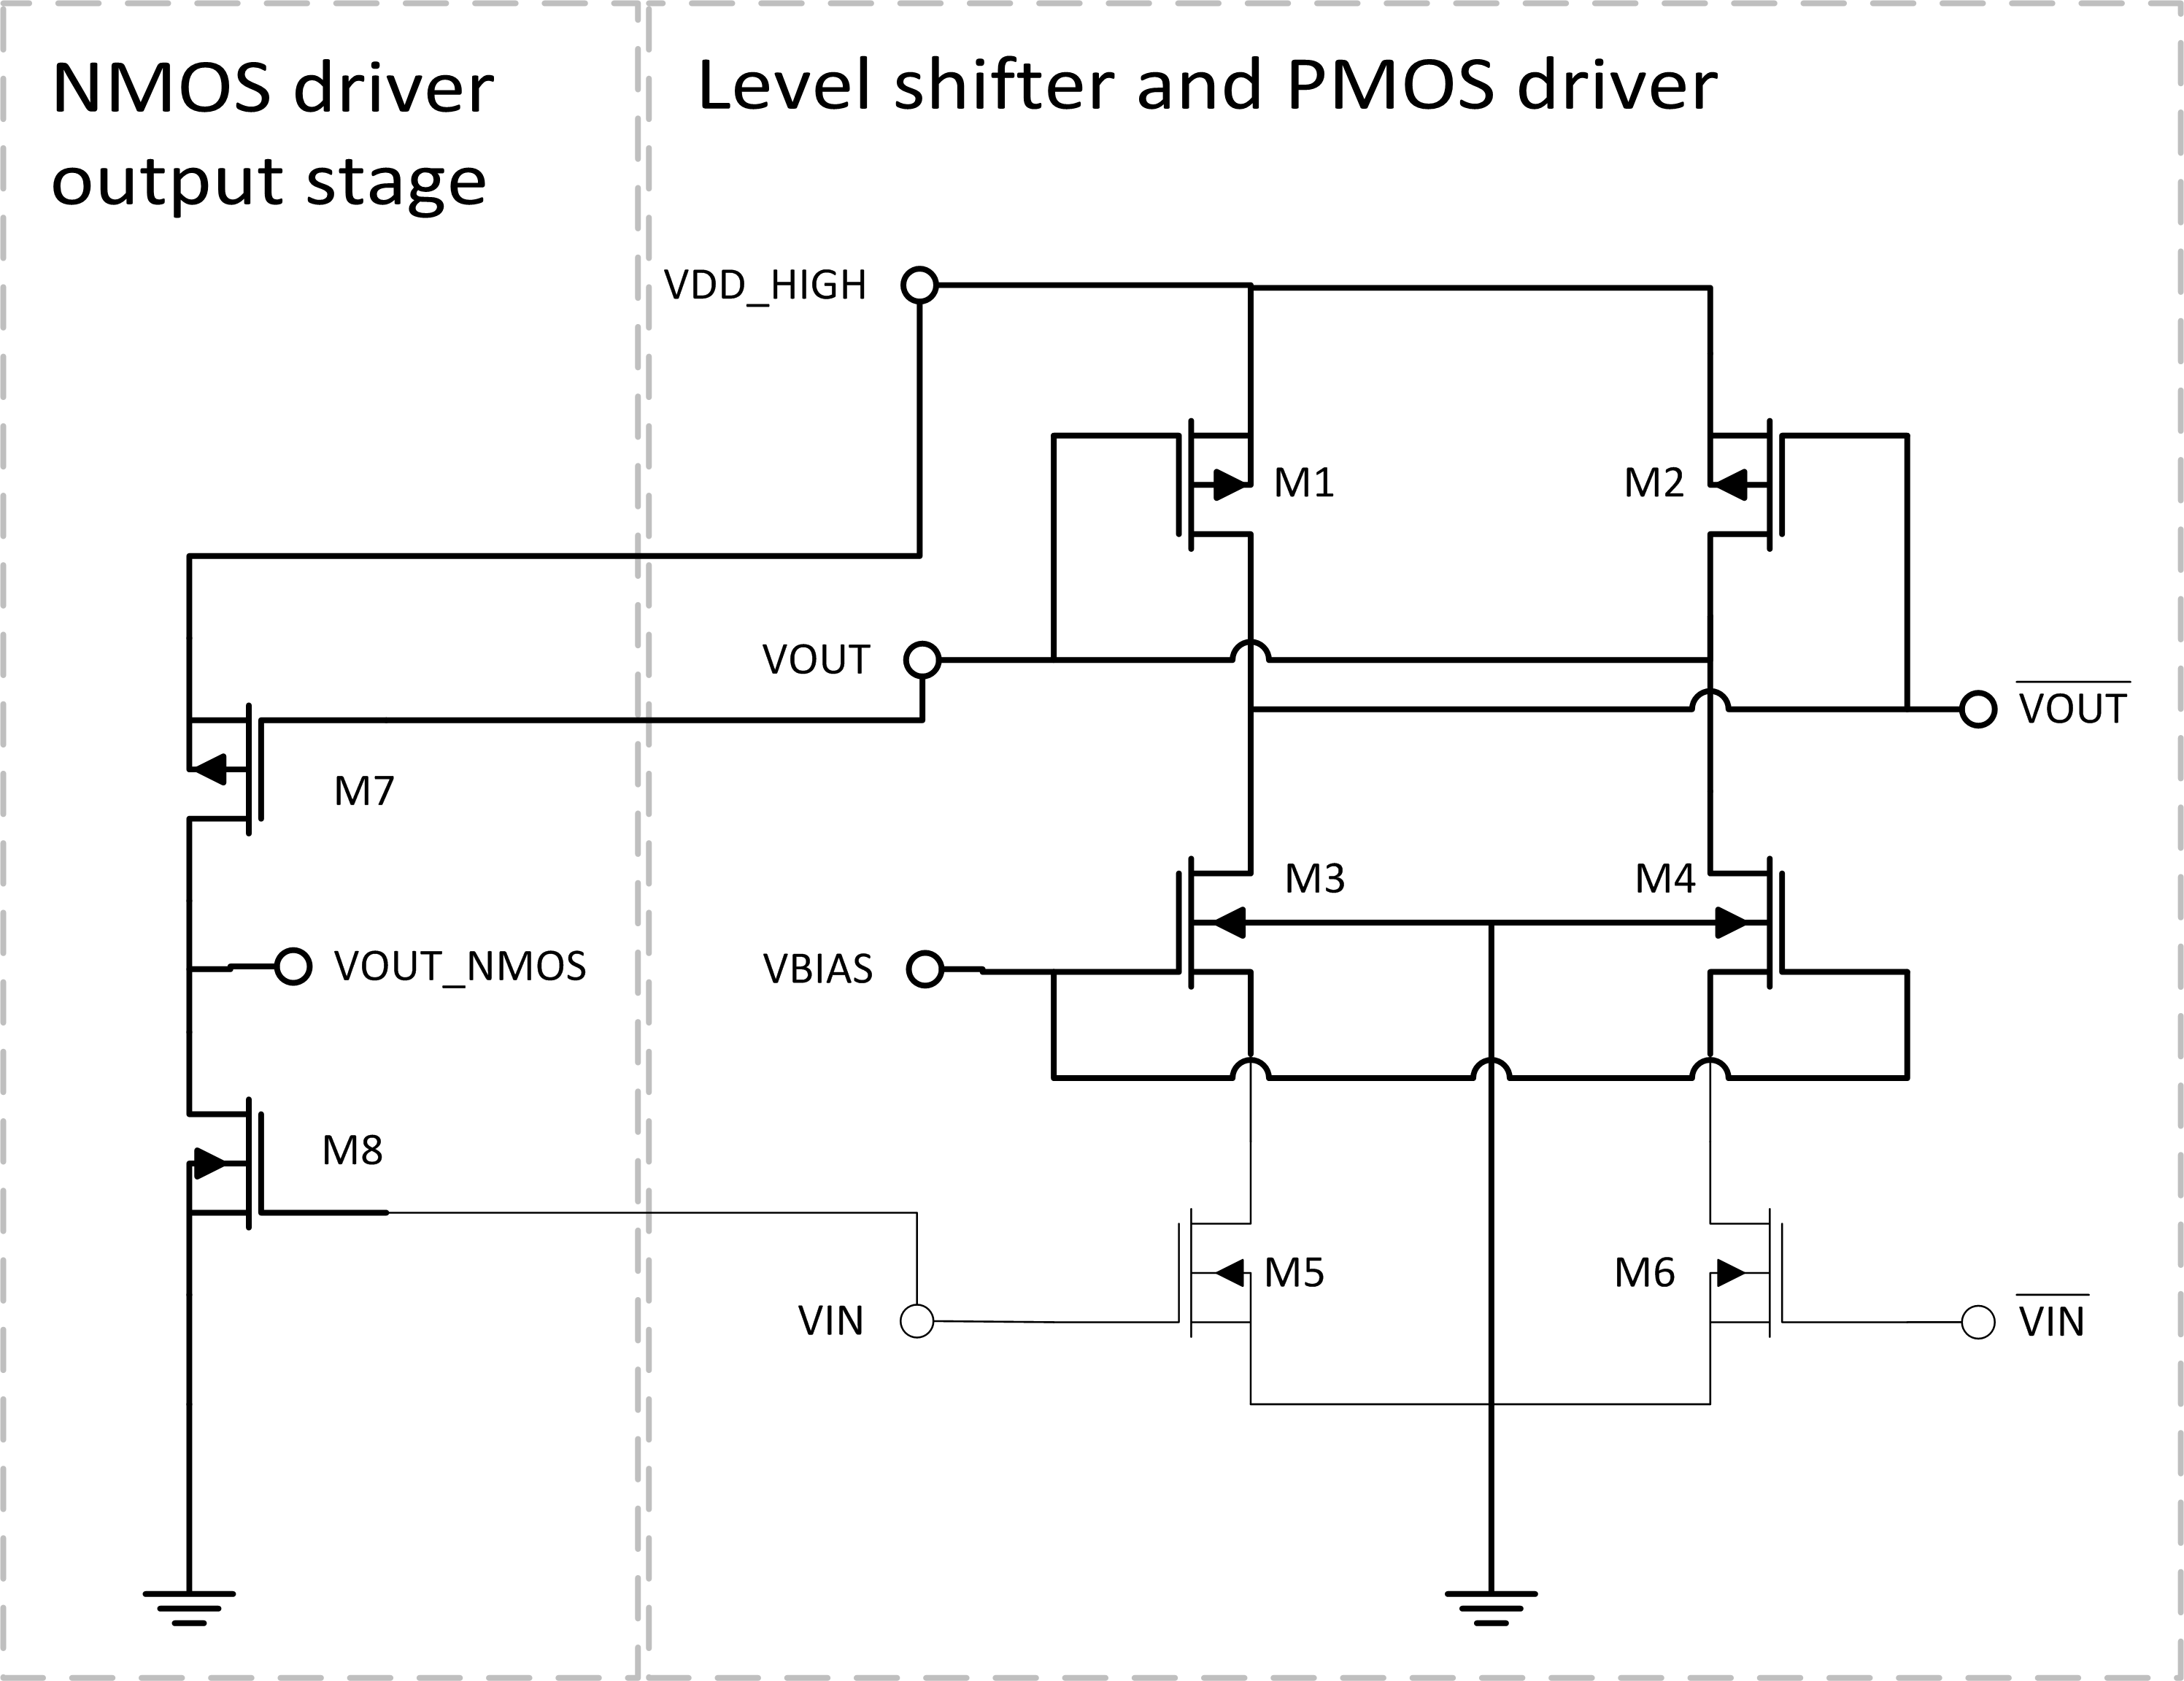
\includegraphics[width=0.5\textwidth]{levelshifter_schematic}
 \caption{Schematics of the levelshifter, thick wires indicate a high voltage regime and thing the low voltage transistors}
 \label{fig:schematic_levelshifter}
\end{figure}
The chosen design is a modified version of the one proposed in~\cite{powerdac} and is shown in Fig.~\ref{fig:schematic_levelshifter}. The inputs are connected to the gates of the low voltage transistors M5 and M6 and have an input range of 0V(off) to 1.1V(on). For correct operation VIN and \textoverline{VIN} must be each other's logical inverse. VBIAS is set to ??V and is connected to the gates of M3 and M4. These transistors protect M5 and M6 from the high supply voltage. M1 and M2 provide an positive feed back loop, which makes the circuit function. Its operation is explained using a low to high transition, so initially VIN is 0V, \textoverline{VIN} is 1.1V, VOUT is on its off value and \textoverline{VOUT} is 2V. In this situation only the right branch is conducting current, because \textoverline{VIN} is high and since there is no current in the left branch \textoverline{VOUT} is low. When VIN transitions to a high state, it starts conducting current, forcing VM5 to go a bit higher, as well as \textoverline{VOUT}. Because \textoverline{VOUT} increases, the current through the right branch decreases as well as VOUT. The decreased VOUT makes the left branch conduct more current and \textoverline{VOUT} go higher. Due to this postive feedback loop VOUT will go to VDD. To drive the NMOS transistors the levelshifter also needs another output stage, which can consist of a thick oxide PMOS and an NMOS transistor. the PMOS will be driven by VOUT and the NMOS by VIN. To gether the can rase the ON voltage to 2V compared to the output voltage of 1.1V from the low voltage transistors. 

A parameter sweep is shown in Fig.~\ref{fig:levelshifter_sweep}. It shows that the circuit should be able to function. The sweep is simulated while the level shifter is driving the gate of a thick oxide PMOS transistor that is 60 $\mu$m wide and 300 nm long. In this sweep the width of transistor M2 is swept from 30 to 60 $\mu$m and it shows the impact of this parameter on the rise time. Using this simulation the width of M2 is chosen to be 45 $\mu$m, because it sets the on voltage close to the desired 3V and the difference in risetime compared to larger widths is very small. However, to meet the requirments of a 2 GHz LO frequency, the circuit still must become significantly faster.
\begin{figure}[h]
 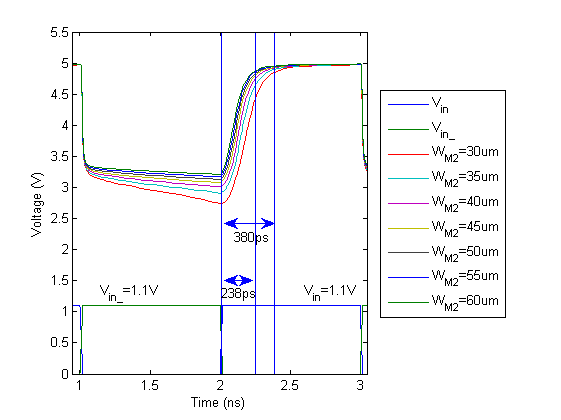
\includegraphics[width=0.5\textwidth]{lvlshift_sweep_wP2}
 \caption{Early simulation results of the levelshifter}
 \label{fig:levelshifter_sweep}
\end{figure}

A final aspect of interest is the power consumption of the levelshifter. This is determined mostly by the current necessary for driving the load transistor. The gates of the load are both charged and discharged via the levelshifter, causing most of the powerconsumption. But also the levelshifter's transistors are relatively large and cost significant power to switch. Simulation results are not avaiable yet. 